\clearpage

\chapter{\documentName}
\section{\documentName}

\testimonial

The original assignment can be found \pdflink{\AssDir Assignment 3A - Instruction.pdf}{here} and \pdflink{\AssDir Assignment 3B - Games.pdf}{here}.

% Problem 1
\begin{problem}{Problem 1}
    \begin{statement}{Problem Statement}
        Consider the zero-sum game tree shown below. Triangles that point up, such as at the top node (root), represent choices for the maximizing player; triangles that point down represent choices 
        for the minimizing player. Assuming both players act optimally, fill in the minimax value of each node.

        \begin{center}
            \begin{tikzpicture}
                % Upward facing triangles
                \tikzstyle{upward} = [regular polygon, regular polygon sides=3, minimum size=1.5cm, draw]
                \tikzstyle{downward} = [regular polygon, regular polygon sides=3, minimum size=1.5cm, draw, shape border rotate=180]
                \tikzstyle{square} = [rectangle, minimum size=0.75cm, draw]

                % Root Node
                \node[upward] (root) at (0,0) {};
                % Children of the root node
                \node[downward] (rootLeft) at (-3,-2) {};
                \node[downward] (rootMid) at (0,-2) {};
                \node[downward] (rootRight) at (3,-2) {};
                % Grandchildren of the root node
                \node[square] (rootLeftLeft) at (-4,-4) {10};
                \node[square] (rootLeftMid) at (-3,-4) {8};
                \node[square] (rootLeftRight) at (-2,-4) {3};
                \node[square] (rootMidLeft) at (-1,-4) {2};
                \node[square] (rootMidMid) at (0,-4) {15};
                \node[square] (rootMidRight) at (1,-4) {7};
                \node[square] (rootRightLeft) at (2,-4) {6};
                \node[square] (rootRightMid) at (3,-4) {5};
                \node[square] (rootRightRight) at (4,-4) {4};

                % Edges
                \draw (root) -- (rootLeft);
                \draw (root) -- (rootMid);
                \draw (root) -- (rootRight);
                \draw (rootLeft) -- (rootLeftLeft);
                \draw (rootLeft) -- (rootLeftMid);
                \draw (rootLeft) -- (rootLeftRight);
                \draw (rootMid) -- (rootMidLeft);
                \draw (rootMid) -- (rootMidMid);
                \draw (rootMid) -- (rootMidRight);
                \draw (rootRight) -- (rootRightLeft);
                \draw (rootRight) -- (rootRightMid);
                \draw (rootRight) -- (rootRightRight);
            \end{tikzpicture}
        \end{center}
    \end{statement}

    \clearpage

    \begin{highlight}[Solution]
        When we say `minimizing player', we are constituting that that given player must pick the minimum value amongst its children. So the triangles that point down must pick the minimum value from
        its children. Conversely, the `maximizing player must pick the maximum value from its children. 

        We first start by finding the minimum value of all the downward facing triangles, and then once this is completed, we pick the maximum value from the downward facing triangles for the root node
        (the upward facing triangle.)

        \begin{center}
            \begin{tikzpicture}
                % Upward facing triangles
                \tikzstyle{upward} = [regular polygon, regular polygon sides=3, minimum size=1.5cm, draw]
                \tikzstyle{downward} = [regular polygon, regular polygon sides=3, minimum size=1.5cm, draw, shape border rotate=180]
                \tikzstyle{square} = [rectangle, minimum size=0.75cm, draw]

                % Root Node
                \node[upward] (root) at (0,0) {4};
                % Children of the root node
                \node[downward] (rootLeft) at (-3,-2) {3};
                \node[downward] (rootMid) at (0,-2) {2};
                \node[downward] (rootRight) at (3,-2) {4};
                % Grandchildren of the root node
                \node[square] (rootLeftLeft) at (-4,-4) {10};
                \node[square] (rootLeftMid) at (-3,-4) {8};
                \node[square] (rootLeftRight) at (-2,-4) {3};
                \node[square] (rootMidLeft) at (-1,-4) {2};
                \node[square] (rootMidMid) at (0,-4) {15};
                \node[square] (rootMidRight) at (1,-4) {7};
                \node[square] (rootRightLeft) at (2,-4) {6};
                \node[square] (rootRightMid) at (3,-4) {5};
                \node[square] (rootRightRight) at (4,-4) {4};

                % Edges
                \draw (root) -- (rootLeft);
                \draw (root) -- (rootMid);
                \draw (root) -- (rootRight);
                \draw (rootLeft) -- (rootLeftLeft);
                \draw (rootLeft) -- (rootLeftMid);
                \draw (rootLeft) -- (rootLeftRight);
                \draw (rootMid) -- (rootMidLeft);
                \draw (rootMid) -- (rootMidMid);
                \draw (rootMid) -- (rootMidRight);
                \draw (rootRight) -- (rootRightLeft);
                \draw (rootRight) -- (rootRightMid);
                \draw (rootRight) -- (rootRightRight);
            \end{tikzpicture}
        \end{center}
    \end{highlight}
\end{problem}

% Problem 2
\begin{problem}{Problem 2}
    \begin{statement}{Problem Statement}
        Which nodes can be pruned from the game tree above through alpha-beta pruning? If no nodes can be pruned, explain why not. Assume the search goes from left to right; when choosing which child 
        to visit first, choose the left-most unvisited child.
    \end{statement}

    \clearpage

    \begin{highlight}[Solution]
        In the leftmost subtree, we evaluate the values 10, 8, and 3. Alpha is updated to 10 and beta is updated to 3 after evaluating these nodes

        In the middle subtree, since alpha was previously set to 10, when we evaluate 2, beta is updated to 2. As beta is now less than or equal to alpha, further nodes in this subtree (15 and 7) are pruned.
        
        In the rightmost subtree, alpha remains 10 and beta remains 2. Evaluating the nodes with values 6, 5, and 4 does not result in any updates that would trigger further pruning. Therefore, no 
        values are pruned from this subtree.
        
        The nodes that are pruned are those in the middle subtree with values 15 and 7. This is because, with alpha set to 10, beta is continuously updated to smaller values, leading to the pruning of 
        larger values as they are no longer relevant to the optimal decision-making process.
        
        \begin{center}
            \begin{highlightenv}[10cm]
                \begin{center}
                    Nodes \textbf{15} and \textbf{7} are pruned.
                \end{center}
            \end{highlightenv}
        \end{center}
    \end{highlight}
\end{problem}

% Problem 3
\begin{problem}{Problem 3}
    \begin{statement}{Problem Statement}
        Again, consider the same zero-sum game tree, except that now, instead of a minimizing player, we have a chance node that will select one of the three values uniformly at random. Fill in the 
        expectimax value of each node. The game tree is redrawn below for your convenience.

        \begin{center}
            \begin{tikzpicture}
                % Upward facing triangles
                \tikzstyle{upward} = [regular polygon, regular polygon sides=3, minimum size=1.5cm, draw]
                \tikzstyle{cirlce} = [circle, minimum size=1cm, draw]
                \tikzstyle{square} = [rectangle, minimum size=0.75cm, draw]
    
                % Root Node
                \node[upward] (root) at (0,0) {};
                % Children of the root node
                \node[cirlce] (rootLeft) at (-3,-2) {};
                \node[cirlce] (rootMid) at (0,-2) {};
                \node[cirlce] (rootRight) at (3,-2) {};
                % Grandchildren of the root node
                \node[square] (rootLeftLeft) at (-4,-4) {10};
                \node[square] (rootLeftMid) at (-3,-4) {8};
                \node[square] (rootLeftRight) at (-2,-4) {3};
                \node[square] (rootMidLeft) at (-1,-4) {2};
                \node[square] (rootMidMid) at (0,-4) {15};
                \node[square] (rootMidRight) at (1,-4) {7};
                \node[square] (rootRightLeft) at (2,-4) {6};
                \node[square] (rootRightMid) at (3,-4) {5};
                \node[square] (rootRightRight) at (4,-4) {4};
    
                % Edges
                \draw (root) -- (rootLeft);
                \draw (root) -- (rootMid);
                \draw (root) -- (rootRight);
                \draw (rootLeft) -- (rootLeftLeft);
                \draw (rootLeft) -- (rootLeftMid);
                \draw (rootLeft) -- (rootLeftRight);
                \draw (rootMid) -- (rootMidLeft);
                \draw (rootMid) -- (rootMidMid);
                \draw (rootMid) -- (rootMidRight);
                \draw (rootRight) -- (rootRightLeft);
                \draw (rootRight) -- (rootRightMid);
                \draw (rootRight) -- (rootRightRight);
            \end{tikzpicture}
        \end{center}
    \end{statement}

    \clearpage

    \begin{highlight}[Solution]
        In the context of random chance nodes, we aren't essentially `randomly' selecting a value from the possible children. Instead, we are taking the average of the children and assigning that as 
        the value for the node. If we perform this choice for each subtree, and then take the maximum value from the children of the root node, we can determine the expectimax value of each node in
        this scenario. This scenario can be found below.
        \begin{center}
            \begin{tikzpicture}
                % Upward facing triangles
                \tikzstyle{upward} = [regular polygon, regular polygon sides=3, minimum size=1.5cm, draw]
                \tikzstyle{cirlce} = [circle, minimum size=1cm, draw]
                \tikzstyle{square} = [rectangle, minimum size=0.75cm, draw]
    
                % Root Node
                \node[upward] (root) at (0,0) {8};
                % Children of the root node
                \node[cirlce] (rootLeft) at (-3,-2) {7};
                \node[cirlce] (rootMid) at (0,-2) {8};
                \node[cirlce] (rootRight) at (3,-2) {5};
                % Grandchildren of the root node
                \node[square] (rootLeftLeft) at (-4,-4) {10};
                \node[square] (rootLeftMid) at (-3,-4) {8};
                \node[square] (rootLeftRight) at (-2,-4) {3};
                \node[square] (rootMidLeft) at (-1,-4) {2};
                \node[square] (rootMidMid) at (0,-4) {15};
                \node[square] (rootMidRight) at (1,-4) {7};
                \node[square] (rootRightLeft) at (2,-4) {6};
                \node[square] (rootRightMid) at (3,-4) {5};
                \node[square] (rootRightRight) at (4,-4) {4};
    
                % Edges
                \draw (root) -- (rootLeft);
                \draw (root) -- (rootMid);
                \draw (root) -- (rootRight);
                \draw (rootLeft) -- (rootLeftLeft);
                \draw (rootLeft) -- (rootLeftMid);
                \draw (rootLeft) -- (rootLeftRight);
                \draw (rootMid) -- (rootMidLeft);
                \draw (rootMid) -- (rootMidMid);
                \draw (rootMid) -- (rootMidRight);
                \draw (rootRight) -- (rootRightLeft);
                \draw (rootRight) -- (rootRightMid);
                \draw (rootRight) -- (rootRightRight);
            \end{tikzpicture}
        \end{center}
    \end{highlight}
\end{problem}

% Problem 4
\begin{problem}{Problem 4}
    \begin{statement}{Problem Statement}
        Which nodes can be pruned from the game tree above through alpha-beta pruning?  If no nodes can be pruned, explain why not.
    \end{statement}

    \clearpage

    \begin{highlight}[Solution]
        Since we are using random chance nodes for this problem, we cannot necessarily prune any nodes from the game tree with alpha-beta pruning. This is because the random chance nodes do not
        pick values systematically like the minimizing player in the minimax algorithm. Therefore, we cannot prune any nodes from the game tree using alpha-beta pruning in this scenario.

        \begin{center}
            \begin{highlightenv}[10cm]
                \begin{center}
                    No nodes can be pruned from the game tree.
                \end{center}
            \end{highlightenv}
        \end{center}
    \end{highlight}
\end{problem}

% Problem 5 
\begin{problem}{Problem 5 - Reflex Agent}
    \begin{statement}{Problem Statement}
        Improve the ReflexAgent in \texttt{multiAgents.py} to play respectably. The provided reflex agent code provides some helpful examples of methods that query the GameState for information. A capable 
        reflex agent will have to consider both food locations and ghost locations to perform well. Your agent should easily and reliably clear the testClassic layout:

    \begin{code}[Bash]
    $ python pacman.py -p ReflexAgent -l testClassic
    \end{code}

        Try out your reflex agent on the default \texttt{mediumClassic} layout with one ghost or two (and animation off to speed up the display):

    \begin{code}[Bash]
    $ python pacman.py --frameTime 0 -p ReflexAgent -k 1
    $ python pacman.py --frameTime 0 -p ReflexAgent -k 2
    \end{code}

        How does your agent fare? It will likely often die with 2 ghosts on the default board, unless your evaluation function is quite good. Try the reciprocal of important values (such as distance to food) 
        rather than just the values themselves. The evaluation function you're writing is evaluating state-action pairs; in later parts of the assignment, you'll be evaluating states.

        \textit{Command line options that may be useful:}

        \begin{itemize}
            \item Default ghosts are random; you can also play for fun with slightly smarter directional ghosts using \texttt{-g DirectionalGhost}.
            \item If the randomness is preventing you from telling whether your agent is improving, you can use \texttt{-f} to run with a fixed random seed (same random choices every game).
            \item You can also play multiple games in a row with -n.
            \item Turn off graphics with -q to run lots of games quickly.
        \end{itemize}
        
        \begin{center}
            \begin{highlightenv}[15cm]
                \textbf{Problem 1}. Improve the Pacman ReflexAgent behavior as described above. We will run your agent on the openClassic layout 10 times. You will receive 0 points if your agent times 
                out, or never wins. You will receive 1 point if your agent wins at least 5 times, or 2 points if your agent wins all 10 games. You will receive an addition 1 point if your agent's average 
                score is greater than 500, or 2 points if it is greater than 1000.
            \end{highlightenv}
        \end{center}

        You can try your agent out under these conditions with:

    \begin{code}[Bash]
    $ python autograder.py -q q1
    $ python autograder.py -q q1 --no-graphics # disables graphics
    \end{code}

        Don't spend too much time on this question, though, as the meat of the assignment lies ahead!
    \end{statement}

    \begin{highlight}[Solution]
    \begin{code}[Python]
    class ReflexAgent(Agent):
    """
        A reflex agent chooses an action at each choice point by examining
        its alternatives via a state evaluation function.

        The code below is provided as a guide.  You are welcome to change
        it in any way you see fit, so long as you don't touch our method
        headers.
    """


    def getAction(self, gameState):
        """
        You do not need to change this method, but you're welcome to.

        getAction chooses among the best options according to the evaluation function.

        Just like in the previous project, getAction takes a GameState and returns
        some Directions.X for some X in the set {North, South, West, East, Stop}
        """
        # Collect legal moves and successor states
        legalMoves = gameState.getLegalActions()

        # Choose one of the best actions
        scores = [self.evaluationFunction(gameState, action) for action in legalMoves]
        bestScore = max(scores)
        bestIndices = [index for index in range(len(scores)) if scores[index] == bestScore]
        chosenIndex = random.choice(bestIndices) # Pick randomly among the best

        "Add more of your code here if you want to"

        return legalMoves[chosenIndex]

    """ evaluationFunction is the function that evaluates the current state of the game and returns a score
        Input:
            self - The object pointer
            currentGameState - The current state of the game
            action - The action to be taken
        Algorithm:
            * Get the current position of the pacman
            * Get the food, ghosts and capsules from the current state
            * Calculate the distance of the pacman from the food
            * Iterate over the total number of ghosts
            * If the ghost is scared, add the score
            * If the ghost is not scared, subtract the score
            * Calculate the distance of the pacman from the capsules
            * If the capsule distances are not empty
            * Get the minimum distance of the pacman from the capsules
            * Calculate the score
            * Get the remaining food
            * Subtract the remaining food from the score
            * Calculate the final score
            * Add the score of the current state
            * Add the food score
            * Add the ghost score
            * Add the capsule score
            * Add the food count score
            * Return the final score
        Output:
            finalScore - The score of the current state
    """
    def evaluationFunction(self, currentGameState, action):
        """
        Design a better evaluation function here.

        The evaluation function takes in the current and proposed successor
        GameStates (pacman.py) and returns a number, where higher numbers are better.

        The code below extracts some useful information from the state, like the
        remaining food (newFood) and Pacman position after moving (newPos).
        newScaredTimes holds the number of moves that each ghost will remain
        scared because of Pacman having eaten a power pellet.

        Print out these variables to see what you're getting, then combine them
        to create a masterful evaluation function.
        """
        "*** YOUR CODE HERE ***"
        # Useful information you can extract from a GameState (pacman.py)
        successorGameState = currentGameState.generatePacmanSuccessor(action)
        pacmanPos = successorGameState.getPacmanPosition()
        food = successorGameState.getFood()
        ghosts = successorGameState.getGhostStates()
        capsules = currentGameState.getCapsules()
        # Initialize the variables
        foodScore = 0
        ghostScore = 0
        capsuleScore = 0
        foodDistances = [manhattanDistance(pacmanPos, foodPos) for foodPos in food.asList()]
        # If the food distances are not empty
        if foodDistances:
            nearestFoodDist = min(foodDistances)  # Get the minimum distance of the pacman from the food
            foodScore = 1.0 / nearestFoodDist # Calculate the score
        # Iterate over the total number of ghosts
        for ghost in ghosts:
            ghostDist = manhattanDistance(pacmanPos, ghost.getPosition()) # Calculate the distance of the pacman from the ghosts
            # If the ghost is scared, add the score
            if ghost.scaredTimer > 0:
                ghostScore += 2.0 / (ghostDist + 1)
            # Otherwise, subtract the score
            else:
                ghostScore -= 1.0 / (ghostDist + 1)
        # Calculate the distance of the pacman from the capsules
        capsuleDistances = [manhattanDistance(pacmanPos, capsule) for capsule in capsules]
        # If the capsule distances are not empty
        if capsuleDistances:
            nearestCapsuleDist = min(capsuleDistances)  # Get the minimum distance of the pacman from the capsules
            capsuleScore = 1.0 / (nearestCapsuleDist + 1) # Calculate the score
        # Get the remaining food
        remainingFood = len(food.asList())
        # Subtract the remaining food from the score
        foodCountScore = -remainingFood
        # Calculate the final score
        finalScore = (
            successorGameState.getScore() +
            foodScore * 10 +                 
            ghostScore * 20 +                
            capsuleScore * 10 +              
            foodCountScore * 5               
        )
        return finalScore
    \end{code}
    \end{highlight}
\end{problem}

% Problem 6
\begin{problem}{Problem 6 - Minimax Agent}
    \begin{statement}{Problem Statement}
        Now you will write an adversarial search agent in the provided \texttt{MinimaxAgent} class stub in \texttt{multiAgents.py}. Your minimax agent should work with any number of ghosts, so you'll have to 
        write an algorithm that is slightly more general than what you've previously seen in lecture. In particular, your minimax tree will have multiple min layers (one for each ghost) for every max layer.

        Your code should also expand the game tree to an arbitrary depth. Score the leaves of your minimax tree with the supplied \texttt{self.evaluationFunction}, which defaults to \texttt{scoreEvaluationFunction}. 
        \texttt{MinimaxAgent} extends \texttt{MultiAgentSearchAgent}, which gives access to \texttt{self.depth} and \texttt{self.evaluationFunction}. Make sure your minimax code makes reference to these two 
        variables where appropriate as these variables are populated in response to command line options. It's worth noting that a single search ply is considered to be one Pacman move and all the ghosts' 
        responses, so depth 2 search will involve Pacman and each ghost moving two times.

        \begin{center}
            \begin{highlightenv}[15cm]
                Problem 2. Using your adversarial search agent in the class above, we will be checking your code to determine whether it explores the correct number of game states. This is the only way 
                reliable way to detect some very subtle bugs in implementations of minimax. As a result, the autograder will be very picky about how many times you call \texttt{GameState.generateSuccessor}. 
                If you call it any more or less than necessary, the autograder will mark your code incorrect.
            \end{highlightenv}
        \end{center}

        To test and debug your code, run \texttt{python autograder.py -q q2} (remember from 1.1 how to run it without graphics, too!). This will show what your algorithm does on a number of small trees, as 
        well as a pacman game. The correct implementation of minimax will lead to Pacman losing the game in some tests. This is not a problem: as it is correct behaviour, it will pass the tests. The 
        evaluation function for the Pacman test in this part is already written (\texttt{self.evaluationFunction}). You shouldn't change this function, but recognize that now we're evaluating states rather 
        than actions, as we were for the reflex agent. Look-ahead agents evaluate future states whereas reflex agents evaluate actions from the current state.

        \begin{itemize}
            \item The minimax values of the initial state in the \texttt{minimaxClassic} layout are 9, 8, 7, -492 for depths 1, 2, 3 and 4 respectively. Note that your minimax agent will often win 
            (665/1000 games for us) despite the dire prediction of depth 4 minimax (e.g. \texttt{python pacman.py -p MinimaxAgent -l minimaxClassic -a depth=4}).
            \item Pacman is always agent 0, and the agents move in order of increasing agent index
            \item All states in minimax should be GameStates, either passed in to getAction or generated via \texttt{GameState. generateSuccessor}. In this problem, you will not be abstracting to simplified states.
            \item On larger boards such as \texttt{openClassic} and \texttt{mediumClassic} (the default), you'll find Pacman to be good at not dying, but quite bad at winning. He'll often thrash around 
            without making progress. He might even thrash around right next to a dot without eating it because he doesn't know where he'd go after eating that dot. Don't worry if you see this behavior, 
            question 5 will clean up all of these issues.
            \item When Pacman believes that his death is unavoidable, he will try to end the game as soon as possible because of the constant penalty for living. Sometimes, this is the wrong thing to 
            do with random ghosts, but minimax agents always assume the worst: \texttt{python pacman.py -p MinimaxAgent -l trappedClassic -a depth=3}. Make sure you understand why Pacman rushes the 
            closest ghost in this case.
        \end{itemize}
    \end{statement}

    \begin{highlight}[Solution]
    \begin{code}[Python]
    class MinimaxAgent(MultiAgentSearchAgent):
    """
        Your minimax agent (question 2)
    """
    def getAction(self, gameState):
        """
        Returns the minimax action from the current gameState using self.depth
        and self.evaluationFunction.

        Here are some method calls that might be useful when implementing minimax.

        gameState.getLegalActions(agentIndex):
            Returns a list of legal actions for an agent
            agentIndex=0 means Pacman, ghosts are >= 1

        gameState.generateSuccessor(agentIndex, action):
            Returns the successor game state after an agent takes an action

        gameState.getNumAgents():
            Returns the total number of agents in the game
        """
        "*** YOUR CODE HERE ***"
        """ minimax - Calculates the minimax value of the current state
                Input:
                agentIndex - The index of the agent
                depth - The depth of the search
                gameState - The current state of the game
                Algorithm:
                * If the game is won or lost or the depth is reached
                    * Return the evaluation function of the current state
                * If the agent index is 0
                    * Return the max value
                * Otherwise
                    * Return the min value
                Output:
                The minimax value of the current state
        """
        def minimax(agentIndex, depth, gameState):
            # If the game is won or lost or the depth is reached
            if gameState.isWin() or gameState.isLose() or depth == self.depth:
                return self.evaluationFunction(gameState), None
            # If the agent index is 0
            if agentIndex == 0:
                return maxValue(agentIndex, depth, gameState)
            # Otherwise
            else:
                return minValue(agentIndex, depth, gameState)
        """ maxValue - Calculates the max value of the current state
                Input:
                agentIndex - The index of the agent
                depth - The depth of the search
                gameState - The current state of the game
                Algorithm:
                * Initialize the variables
                * Iterate over the legal actions of the agent
                    * Get the successor of the current state
                    * Calculate the value of the successor
                    * If the value is greater than the max value
                    * Update the max value
                    * Update the best action
                * If the depth is 0
                    * Return the max value and the best action
                * Otherwise
                    * Return the max value
                Output:
                The max value of the current state
        """
        def maxValue(agentIndex, depth, gameState):
            # Initialize the variables
            v = float("-inf")
            bestAction = None
            # Iterate over the legal actions of the agent
            for action in gameState.getLegalActions(agentIndex):
                # Get the successor of the current state
                successor = gameState.generateSuccessor(agentIndex, action)
                # Calculate the value of the successor
                value, _ = minimax((agentIndex + 1) % gameState.getNumAgents(), depth + ((agentIndex + 1) // gameState.getNumAgents()), successor)
                # If the value is greater than the max value
                if value > v:
                    v = value
                    bestAction = action
            # If the depth is 0
            if depth == 0:
                return v, bestAction
            # Otherwise
            else:
                return v, None
        """ minValue - Calculates the min value of the current state
                Input:
                agentIndex - The index of the agent
                depth - The depth of the search
                gameState - The current state of the game
                Algorithm:
                * Initialize the variables
                * Iterate over the legal actions of the agent
                    * Get the successor of the current state
                    * Calculate the value of the successor
                    * If the value is less than the min value
                    * Update the min value
                * Return the min value
                Output:
                The min value of the current state
        """
        def minValue(agentIndex, depth, gameState):
            # Initialize the variables
            v = float("inf")
            # Iterate over the legal actions of the agent
            for action in gameState.getLegalActions(agentIndex):
                # Get the successor of the current state
                successor = gameState.generateSuccessor(agentIndex, action)
                # Calculate the value of the successor
                value, _ = minimax((agentIndex + 1) % gameState.getNumAgents(), depth + ((agentIndex + 1) // gameState.getNumAgents()), successor)
                # If the value is less than the min value
                if value < v:
                    v = value
            return v, None
        # Initialize the variables
        _, action = minimax(0, 0, gameState)
        # Return the action
        return action
    \end{code}
    \end{highlight}
\end{problem}

% Problem 7
\begin{problem}{Problem 7 - Alpha-Beta Pruning}
    \begin{statement}{Problem Statement}
        Make a new agent that uses alpha-beta pruning to more efficiently explore the minimax tree, in \texttt{AlphaBetaAgent}. Again, your algorithm will be slightly more general than the pseudocode 
        from lecture, so part of the challenge is to extend the alpha-beta pruning logic appropriately to multiple minimizer agents. The pseudo-code below represents the algorithm you should implement 
        for this question.

        \begin{center}
            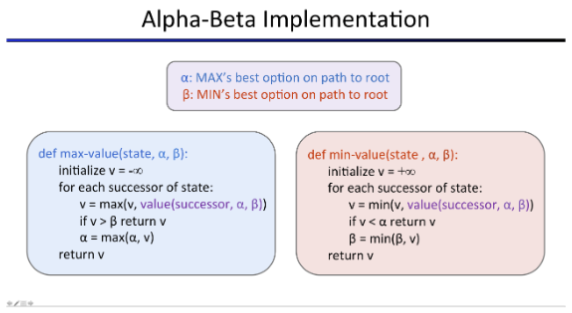
\includegraphics[width=0.5\textwidth]{Images/Alpha Beta.png}
        \end{center}
        You should see a speed-up (perhaps depth 3 alpha-beta will run as fast as depth 2 minimax). Ideally, depth 3 on \texttt{smallClassic} should run in just a few seconds per move or faster: 
        \texttt{python pacman.py -p AlphaBetaAgent -a depth=3 -l smallClassic}.

        The \texttt{AlphaBetaAgent} minimax values should be identical to the \texttt{MinimaxAgent} minimax values, although the actions it selects can vary because of different tie-breaking behavior. 
        Again, the minimax values of the initial state in the \texttt{minimaxClassic} layout are 9, 8, 7 and -492 for depths 1, 2, 3 and 4 respectively.

        \begin{center}
            \begin{highlightenv}[15cm]
                \textbf{Problem 3}. Play the game with your new agent in \texttt{AlphaBetaAgent}. We will test your code on a number of small trees, as well as a pacman game. Because we check your code 
                to determine whether it explores the correct number of states, it is important that you perform alpha-beta pruning without reordering children. In other words, successor states should 
                always be processed in the order returned by \texttt{GameState.getLegalActions}. Again, do not call \texttt{GameState.generateSuccessor} more than necessary.
            \end{highlightenv}
        \end{center}

        You must not prune on equality in order to match the set of states explored by our autograder. Indeed, alternatively, but incompatible with our autograder, would be to also allow for pruning 
        on equality and invoke alpha-beta once on each child of the root node, but this will not match the autograder. The correct implementation of alpha-beta pruning will lead to Pacman losing some 
        of the tests. This is not a problem: as it is correct behavior, it will pass the tests
    \end{statement}

    \begin{highlight}[Solution]
    \begin{code}[Python]
    class AlphaBetaAgent(MultiAgentSearchAgent):
    """
        Your minimax agent with alpha-beta pruning (question 3)
    """
    def getAction(self, gameState):
        """
            Returns the minimax action using self.depth and self.evaluationFunction
        """
        "*** YOUR CODE HERE ***"
        """ alphaBeta - Calculates the alpha-beta value of the current state
                Input:
                agentIndex - The index of the agent
                depth - The depth of the search
                gameState - The current state of the game
                alpha - The alpha value
                beta - The beta value
                Algorithm:
                * If the game is won or lost or the depth is reached
                    * Return the evaluation function of the current state
                * If the agent index is 0
                    * Return the max value
                * Otherwise
                    * Return the min value
                Output:
                The alpha-beta value of the current state
        """
        def alphaBeta(agentIndex, depth, gameState, alpha, beta):
            # If the game is won or lost or the depth is reached
            if gameState.isWin() or gameState.isLose() or depth == self.depth:
                return self.evaluationFunction(gameState), None
            # If the agent index is 0
            if agentIndex == 0:
                return maxValue(agentIndex, depth, gameState, alpha, beta)
            # Otherwise
            else:
                return minValue(agentIndex, depth, gameState, alpha, beta)
        """ maxValue - Calculates the max value of the current state
                Input:
                agentIndex - The index of the agent
                depth - The depth of the search
                gameState - The current state of the game
                alpha - The alpha value
                beta - The beta value
                Algorithm:
                * Initialize the variables
                * Iterate over the legal actions of the agent
                    * Get the successor of the current state
                    * Calculate the value of the successor
                    * If the value is greater than the max value
                    * Update the max value
                    * Update the best action
                    * If the value is greater than beta
                    * Return the max value and the best action
                    * Update the alpha value
                * If the depth is 0
                    * Return the max value and the best action
                * Otherwise
                    * Return the max value
                Output:
                The max value of the current state
        """
        def maxValue(agentIndex, depth, gameState, alpha, beta):
            # Initialize the variables
            v = float("-inf")
            bestAction = None
            # Iterate over the legal actions of the agent
            for action in gameState.getLegalActions(agentIndex):
                # Get the successor of the current state
                successor = gameState.generateSuccessor(agentIndex, action)
                # Calculate the value of the successor
                value, _ = alphaBeta((agentIndex + 1) % gameState.getNumAgents(), depth + ((agentIndex + 1) // gameState.getNumAgents()), successor, alpha, beta)
                # If the value is greater than the max value
                if value > v:
                    v = value
                    bestAction = action
                # If the value is greater than beta
                if v > beta:
                    return v, bestAction
                # Update the alpha value
                alpha = max(alpha, v)
            # If the depth is 0
            if depth == 0:
                return v, bestAction
            # Otherwise
            else:
                return v, None
        """ minValue - Calculates the min value of the current state
                Input:
                agentIndex - The index of the agent
                depth - The depth of the search
                gameState - The current state of the game
                alpha - The alpha value
                beta - The beta value
                Algorithm:
                * Initialize the variables
                * Iterate over the legal actions of the agent
                    * Get the successor of the current state
                    * Calculate the value of the successor
                    * If the value is less than the min value
                    * Update the min value
                    * If the value is less than alpha
                    * Return the min value
                    * Update the beta value
                * Return the min value
                Output:
                The min value of the current state
        """
        def minValue(agentIndex, depth, gameState, alpha, beta):
            # Initialize the variables
            v = float("inf")
            bestAction = None
            # Iterate over the legal actions of the agent
            for action in gameState.getLegalActions(agentIndex):
                # Get the successor of the current state
                successor = gameState.generateSuccessor(agentIndex, action)
                # Calculate the value of the successor
                value, _ = alphaBeta((agentIndex + 1) % gameState.getNumAgents(), depth + ((agentIndex + 1) // gameState.getNumAgents()), successor, alpha, beta)
                # If the value is less than the min value
                if value < v:
                    v = value
                    bestAction = action
                # If the value is less than alpha
                if v < alpha:
                    return v, bestAction
                # Update the beta value
                beta = min(beta, v)
            return v, None
        # Initialize the variables
        _, action = alphaBeta(0, 0, gameState, float("-inf"), float("inf"))
        # Return the action
        return action
    \end{code}
    \end{highlight}
\end{problem}

% Problem 8
\begin{problem}{Problem 8 - Expectimax Agent}
    \begin{statement}{Problem Statement}
        Minimax and alpha-beta are great, but they both assume that you are playing against an adversary who makes optimal decisions. As anyone who has ever won tic-tac-toe can tell you, this is not 
        always the case. In this question you will implement the \texttt{ExpectimaxAgent}, which is useful for modeling probabilistic behavior of agents who may make suboptimal choices.

        As with the search and constraint satisfaction problems covered so far in this class, the beauty of these algorithms is their general applicability. To expedite your own development, we've 
        supplied some test cases based on generic trees. You can debug your implementation on small the game trees using the command: \texttt{python autograder.py -q q4}. 
        
        Debugging on these small and manageable test cases is recommended and will help you to find bugs quickly. \textit{Make sure when you compute your averages that you use floats. Integer division 
        in Python 2 (if you're using python 2) truncates, so that 1/2 = 0, unlike the case with floats where 1.0/2.0 = 0.5.}

        Once your algorithm is working on small trees, you can observe its success in Pacman. Random ghosts are of course not optimal minimax agents, and so modeling them with minimax search may not 
        be appropriate. \texttt{ExpectimaxAgent}, however will no longer take the min over all ghost actions, but the expectation according to your agent's model of how the ghosts act. To simplify 
        your code, assume you will only be running against an adversary which chooses amongst their \texttt{getLegalActions} uniformly at random. To see how the ExpectimaxAgent behaves in Pacman, run:

    \begin{code}[Bash]
    python pacman.py -p ExpectimaxAgent -l minimaxClassic -a depth=3
    \end{code}

        You should now observe a more cavalier approach in close quarters with ghosts. In particular, if Pacman perceives that he could be trapped but might escape to grab a few more pieces of food, he'll at least try.

        Investigate the results of these two scenarios:

    \begin{code}[Bash]
    python pacman.py -p AlphaBetaAgent -l trappedClassic -a depth=3 -q -n 10
    python pacman.py -p ExpectimaxAgent -l trappedClassic -a depth=3 -q -n 10
    \end{code}

        \begin{center}
            \begin{highlightenv}[15cm]
                \textbf{Problem 4}. We will test your \texttt{ExpectimaxAgent} in the two scenarios listed above.
            \end{highlightenv}
        \end{center}

        You should find that your \texttt{ExpectimaxAgent} wins about half the time, while your \texttt{AlphaBetaAgent} always loses. Make sure you understand why the behavior here differs from the minimax case.
    \end{statement}

    \begin{highlight}[Solution]
    \begin{code}[Python]
    class ExpectimaxAgent(MultiAgentSearchAgent):
    """
        Your expectimax agent (question 4)
    """
    def getAction(self, gameState):
        """
            Returns the expectimax action using self.depth and self.evaluationFunction

            All ghosts should be modeled as choosing uniformly at random from their
            legal moves.
        """
        "*** YOUR CODE HERE ***"
        """ expectimax - Calculates the expectimax value of the current state
                Input:
                agentIndex - The index of the agent
                depth - The depth of the search
                gameState - The current state of the game
                Algorithm:
                * If the game is won or lost or the depth is reached
                    * Return the evaluation function of the current state
                * If the agent index is 0
                    * Return the max value
                * Otherwise
                    * Return the exp value
                Output:
                The expectimax value of the current state
        """
        def expectimax(agentIndex, depth, gameState):
            # If the game is won or lost or the depth is reached
            if gameState.isWin() or gameState.isLose() or depth == self.depth:
                return self.evaluationFunction(gameState), None
            # If the agent index is 0
            if agentIndex == 0:
                return maxValue(agentIndex, depth, gameState)
            # Otherwise
            else:
                return expValue(agentIndex, depth, gameState)
        """ maxValue - Calculates the max value of the current state
                Input:
                agentIndex - The index of the agent
                depth - The depth of the search
                gameState - The current state of the game
                Algorithm:
                * Initialize the variables
                * Iterate over the legal actions of the agent
                    * Get the successor of the current state
                    * Calculate the value of the successor
                    * If the value is greater than the max value
                    * Update the max value
                    * Update the best action
                * If the depth is 0
                    * Return the max value and the best action
                * Otherwise
                    * Return the max value
                Output:
                The max value of the current state
        """
        def maxValue(agentIndex, depth, gameState):
            # Initialize the variables
            v = float("-inf")
            bestAction = None
            # Iterate over the legal actions of the agent
            for action in gameState.getLegalActions(agentIndex):
                # Get the successor of the current state
                successor = gameState.generateSuccessor(agentIndex, action)
                # Calculate the value of the successor
                value, _ = expectimax((agentIndex + 1) % gameState.getNumAgents(), depth + ((agentIndex + 1) // gameState.getNumAgents()), successor)
                # If the value is greater than the max value
                if value > v:
                    v = value
                    bestAction = action
            # If the depth is 0
            if depth == 0:
                return v, bestAction
            # Otherwise
            else:
                return v, None
        """ expValue - Calculates the exp value of the current state
                Input:
                agentIndex - The index of the agent
                depth - The depth of the search
                gameState - The current state of the game
                Algorithm:
                * Initialize the variables
                * Iterate over the legal actions of the agent
                    * Get the successor of the current state
                    * Calculate the value of the successor
                    * Add the value to the total value
                * Return the total value
                Output:
                The exp value of the current state
        """
        def expValue(agentIndex, depth, gameState):
            # Initialize the variables
            v = 0
            actions = gameState.getLegalActions(agentIndex)
            p = 1.0 / len(actions)
            # Iterate over the legal actions of the agent
            for action in actions:
                # Get the successor of the current state
                successor = gameState.generateSuccessor(agentIndex, action)
                # Calculate the value of the successor
                value, _ = expectimax((agentIndex + 1) % gameState.getNumAgents(), depth + ((agentIndex + 1) // gameState.getNumAgents()), successor)
                v += p * value
            return v, None
        # Initialize the variables
        _, action = expectimax(0, 0, gameState)
        # Return the action
        return action
    \end{code}
    \end{highlight}
\end{problem}

% Problem 9
\begin{problem}{Problem 9 - Evaluation Function}
    \begin{statement}{Problem Statement}
        Write a better evaluation function for Pacman in the provided function \texttt{betterEvaluationFunction}. The evaluation function should evaluate states, rather than actions like your reflex 
        agent evaluation function did. You may use any tools at your disposal for evaluation. With depth 2 search, your evaluation function should clear the \texttt{smallClassic} layout with one random 
        ghost more than half the time and still run at a reasonable rate.

        \begin{center}
            \begin{highlightenv}[15cm]
                \textbf{Problem 5}. We will test your \texttt{ExpectimaxAgent} with \texttt{betterEvaluationFunction}. The grader will run your agent on the \texttt{smallClassic} layout 10 times. We will give 
                points to your evaluation function in the following way: if you win at least once without timing out the autograder, you receive 1 points. Any agent not satisfying these criteria will 
                receive 0 points. +1 for winning at least 5 times, +2 for winning all 10 times +1 for an average score of at least 500, +2 for an average score of at least 1000 (including scores on 
                lost games) +1 if your games take on average less than 30 seconds on the autograder machine. The additional points for average score and computation time will only be awarded if you 
                win at least 5 times.
            \end{highlightenv}
        \end{center}

        As for your reflex agent evaluation function, you may want to use the reciprocal of important values (such as distance to food) rather than the values themselves. One way you might want to 
        write your evaluation function is to use a linear combination of features. That is, compute values for features about the state that you think are important, and then combine those features 
        by multiplying them by different values and adding the results together. You might decide what to multiply each feature by based on how important you think it is.
    \end{statement}

    \begin{highlight}[Solution]
    \begin{code}[Python]
    """ betterEvaluationFunction - Calculates the better evaluation function of the current state
        Input:
            currentGameState - The current state of the game
        Algorithm:
          * Useful information from the game state
          * Base score is the current game state score
          * Calculate the reciprocal of the distance to the nearest food
          * Calculate the reciprocal of the distance to the nearest ghost
          * Calculate the reciprocal of the distance to the nearest capsule
          * Calculate remaining food score (negative because more food is worse)
          * Combine all the scores with appropriate weights
          * Return the final score
        Output:
            finalScore - The score of the current state
    """
    def betterEvaluationFunction(currentGameState):
        """
            Your extreme ghost-hunting, pellet-nabbing, food-gobbling, unstoppable
            evaluation function (question 5).
    
            DESCRIPTION: This evaluation function balances the immediate need to avoid
            ghosts, collect food, and consume power pellets. It uses the distances to
            the nearest food, ghost, and power pellet, and the number of remaining food
            pellets to compute a score. The function prioritizes food collection while
            avoiding ghosts, and it seeks power pellets to turn ghosts into vulnerable targets.
        """
        # Useful information from the game state
        pacmanPos = currentGameState.getPacmanPosition()
        food = currentGameState.getFood()
        ghosts = currentGameState.getGhostStates()
        capsules = currentGameState.getCapsules()
        # Base score is the current game state score
        score = currentGameState.getScore()
        # Calculate the reciprocal of the distance to the nearest food
        foodDistances = [manhattanDistance(pacmanPos, foodPos) for foodPos in food.asList()]
        if foodDistances:
            nearestFoodDist = min(foodDistances)
            foodScore = 1.0 / nearestFoodDist
        else:
            foodScore = 0
        # Calculate the reciprocal of the distance to the nearest ghost
        ghostScore = 0
        for ghost in ghosts:
            ghostDist = manhattanDistance(pacmanPos, ghost.getPosition())
            if ghost.scaredTimer > 0:
                ghostScore += 2.0 / (ghostDist + 1)  # Incentivize approaching scared ghosts
            else:
                ghostScore -= 1.0 / (ghostDist + 1)  # Discourage approaching active ghosts
        # Calculate the reciprocal of the distance to the nearest capsule
        capsuleDistances = [manhattanDistance(pacmanPos, capsule) for capsule in capsules]
        if capsuleDistances:
            nearestCapsuleDist = min(capsuleDistances)
            capsuleScore = 1.0 / (nearestCapsuleDist + 1)
        else:
            capsuleScore = 0
        # Calculate remaining food score (negative because more food is worse)
        remainingFood = len(food.asList())
        foodCountScore = -remainingFood
        # Combine all the scores with appropriate weights
        finalScore = (
            score +               
            foodScore * 10 +      
            ghostScore * 20 +     
            capsuleScore * 10 +   
            foodCountScore * 5
        )
        return finalScore
    \end{code}
    \end{highlight}
\end{problem}